%\setcounter{chapter}{6}
\chapter{Beam Test of the RD53 chip for CMS Pixel Detector Upgrade Phase 2}\label{ch:testbeam}


la verdad es que
\begin{figure}[!h]
	\centering
	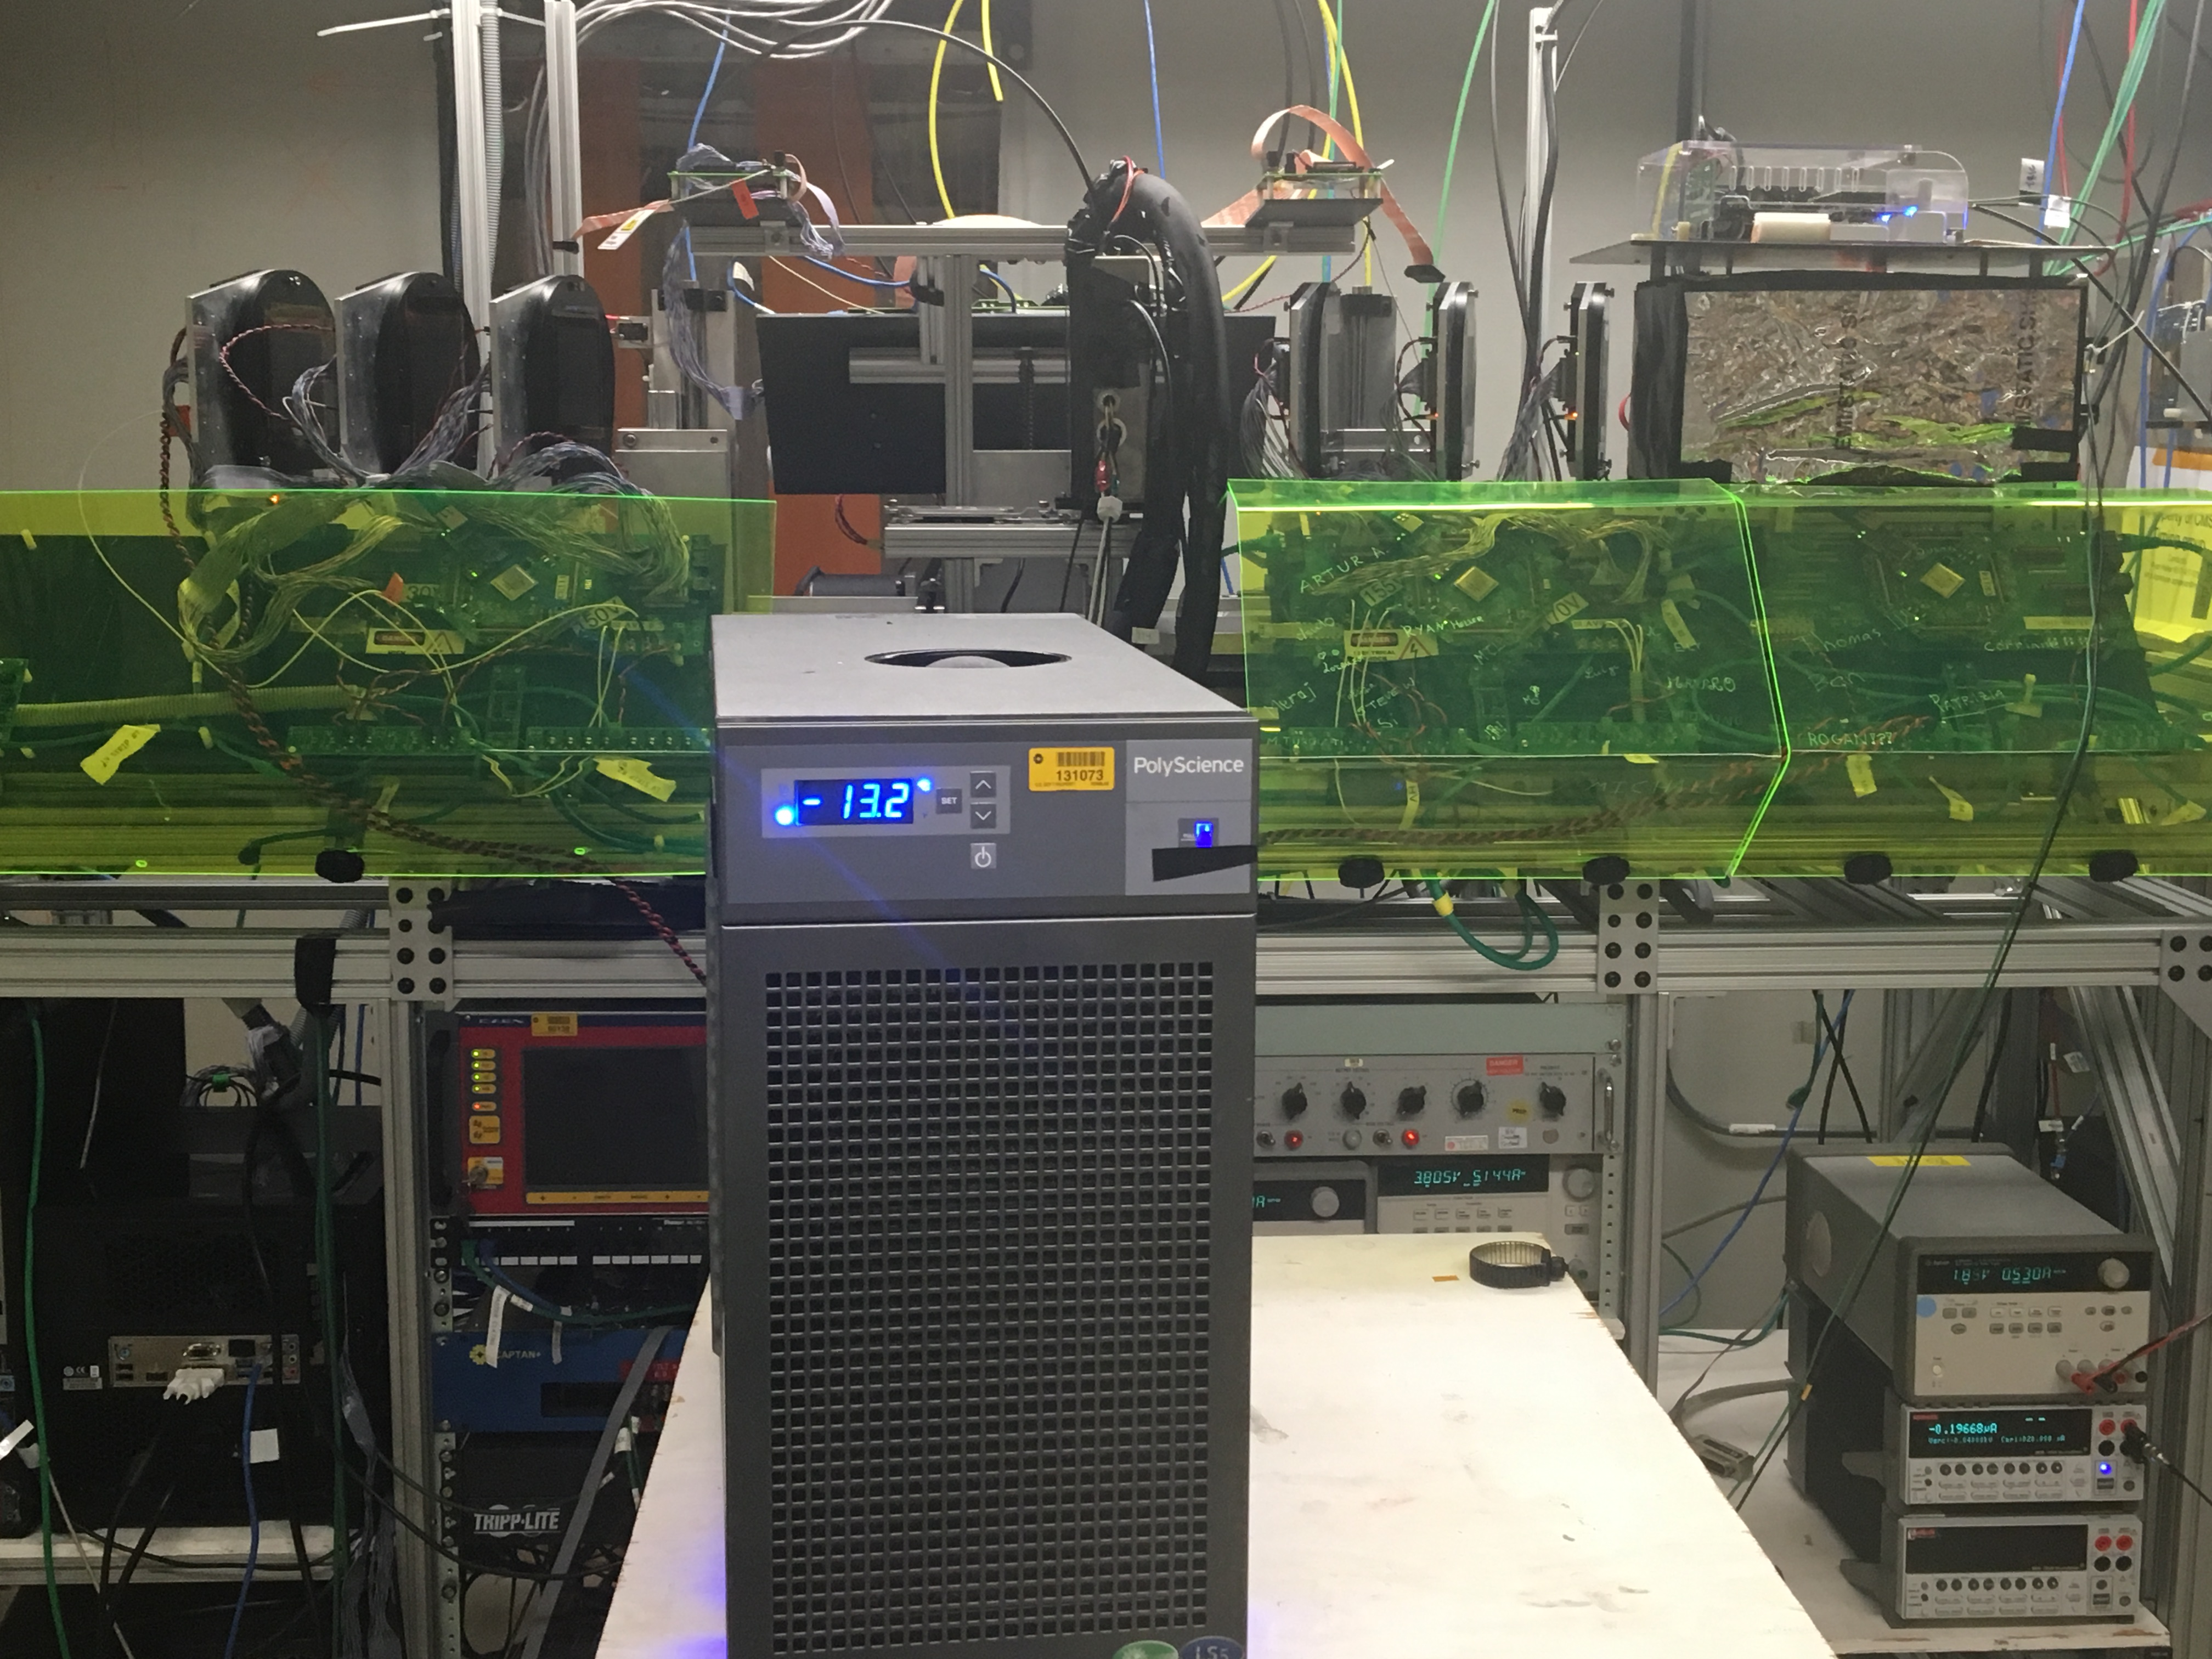
\includegraphics[width=0.6\textwidth]{ch8/ch8_img_setup}
	\caption[Test beam setup] {Test beam setup.}
	\label{ch8imgsetup}
\end{figure}


\begin{figure}[!h]
	\centering
	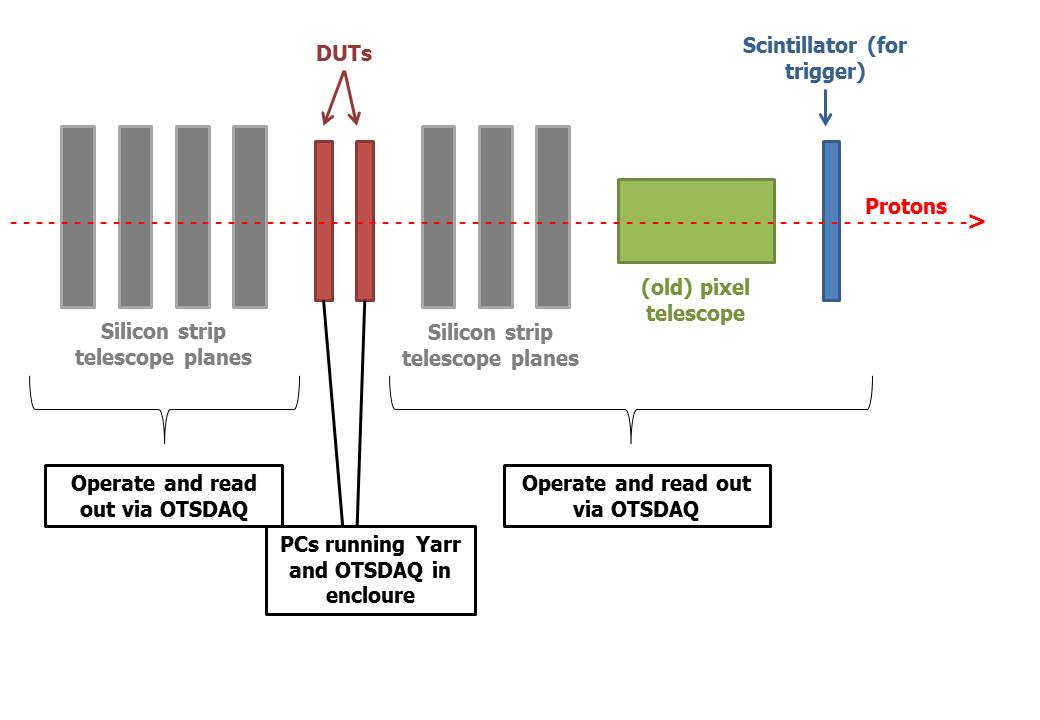
\includegraphics[width=0.6\textwidth]{ch8/ch8_img_setup_2}
	\caption[Test beam setup] {Test beam setup.}
	\label{ch8imgsetup2}
\end{figure}

\begin{figure}[!h]
	\centering
	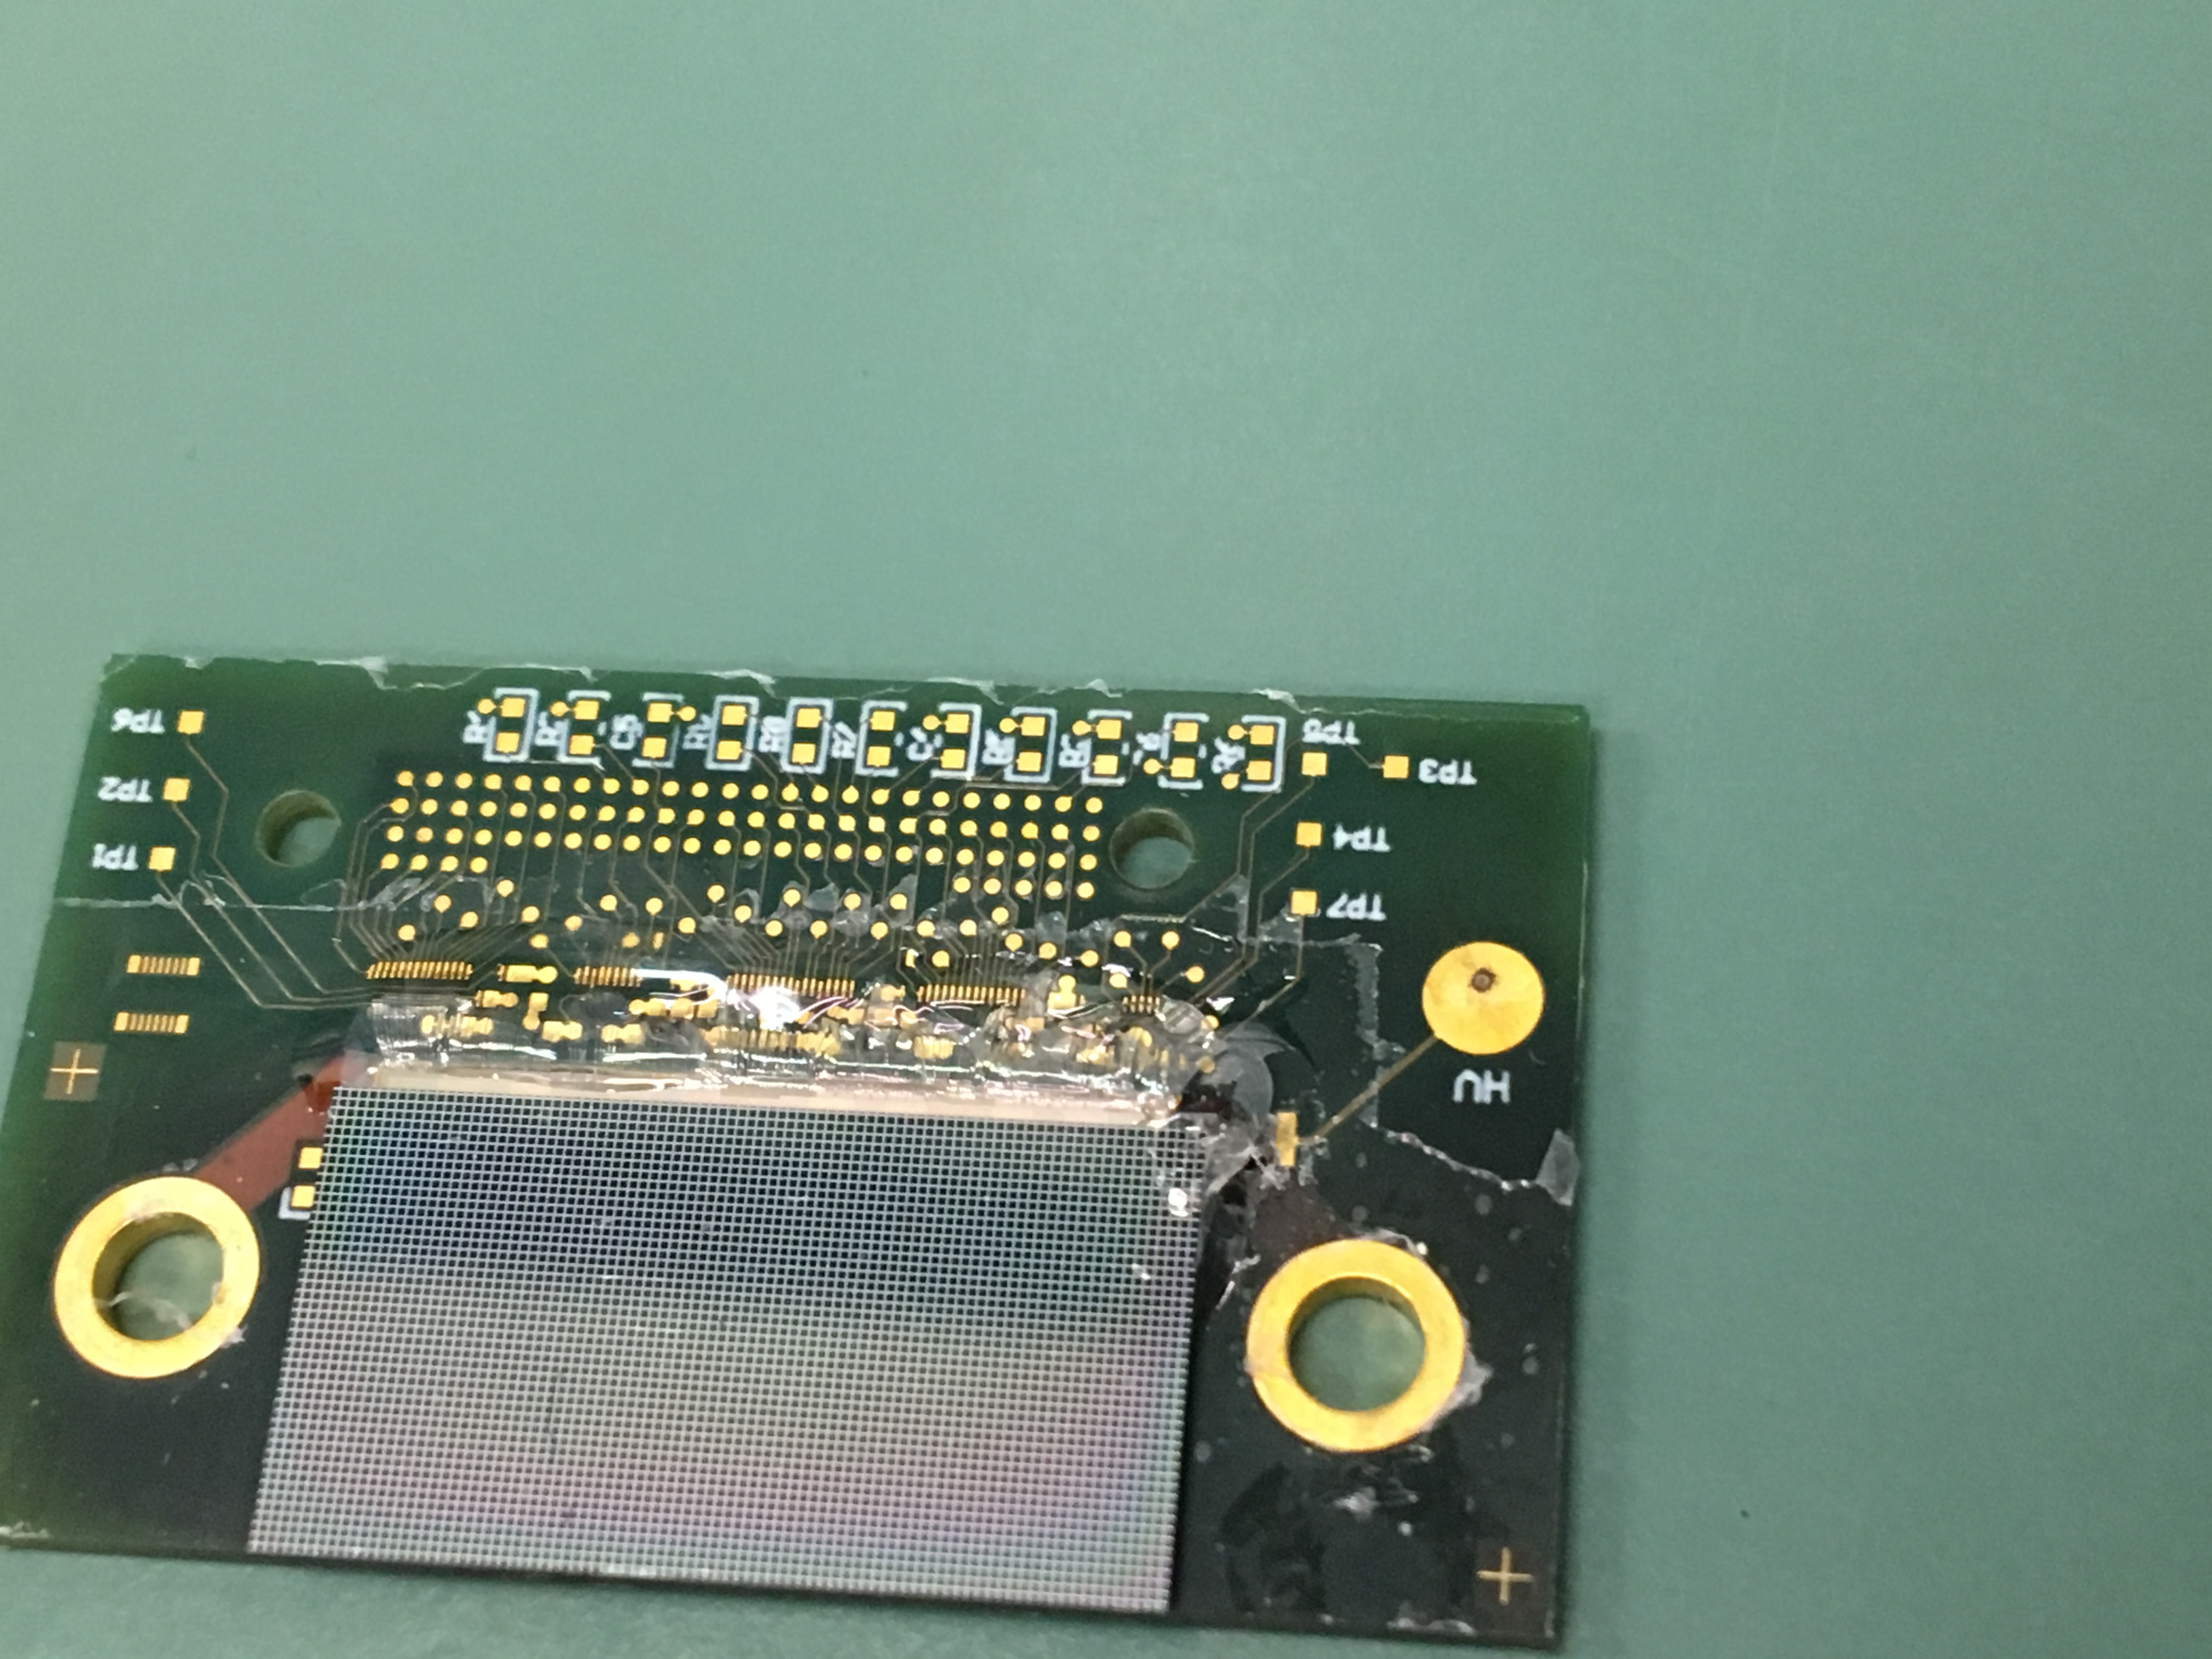
\includegraphics[width=0.6\textwidth]{ch8/ch8_img_chip}
	\caption[chip] {chip.}
	\label{chip}
\end{figure}


\begin{figure}[!h]
	\centering
	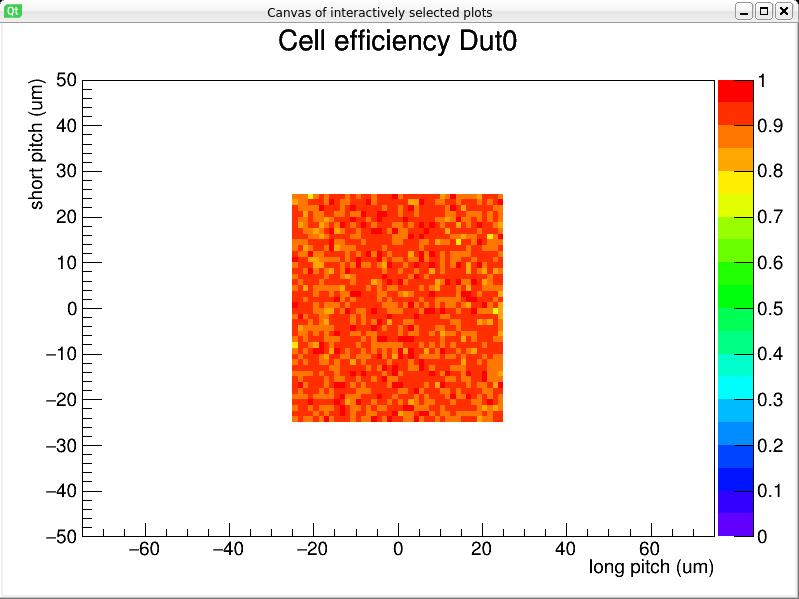
\includegraphics[width=0.6\textwidth]{ch8/ch8_img_celleff}
	\caption[Cell efficiency] {Cell efficiency.}
	\label{celleff}
\end{figure}

\begin{figure}[!h]
	\centering
	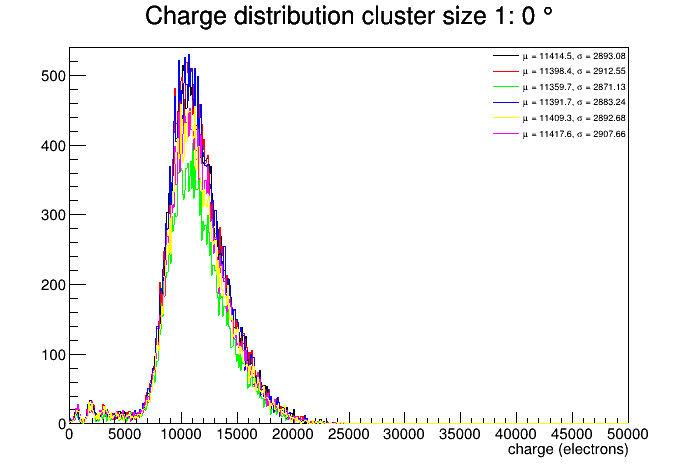
\includegraphics[width=0.6\textwidth]{ch8/ch8_img_charge}
	\caption[Charge] {Charge.}
	\label{charge}
\end{figure}

\begin{figure}[!h]
	\centering
	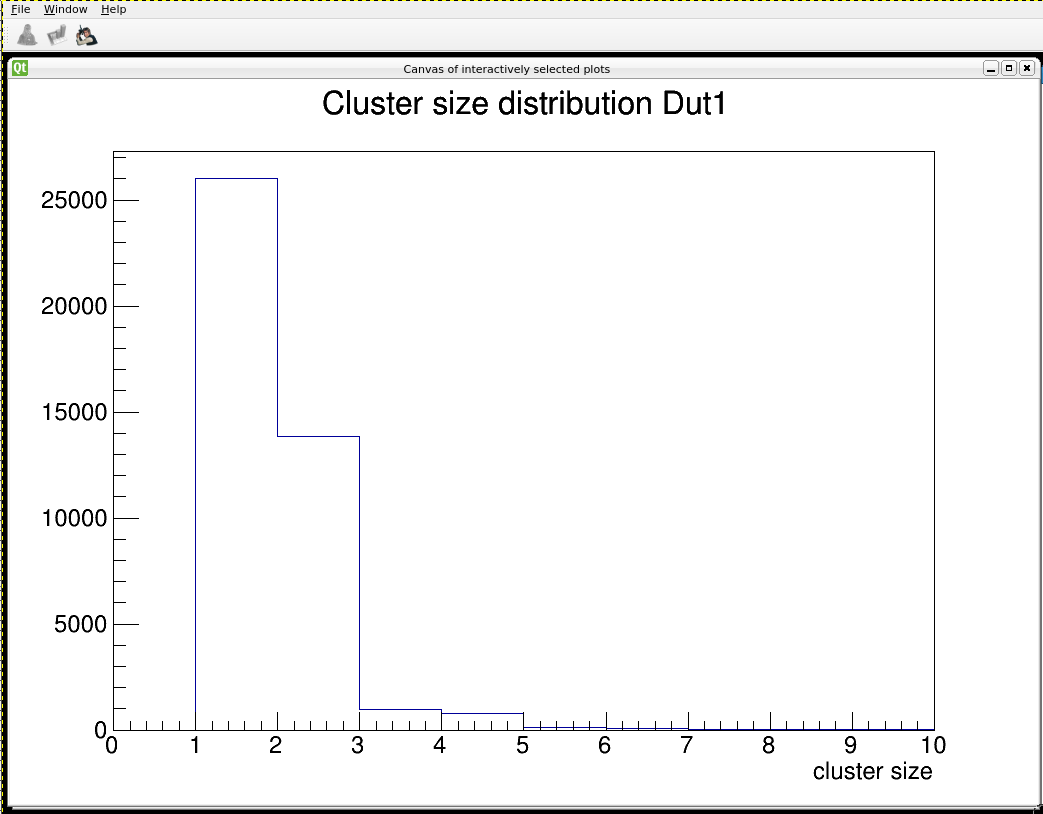
\includegraphics[width=0.6\textwidth]{ch8/ch8_img_cluster}
	\caption[Cluster.] {Cluster.}
	\label{cluster}
\end{figure}

\begin{figure}[!h]
	\centering
	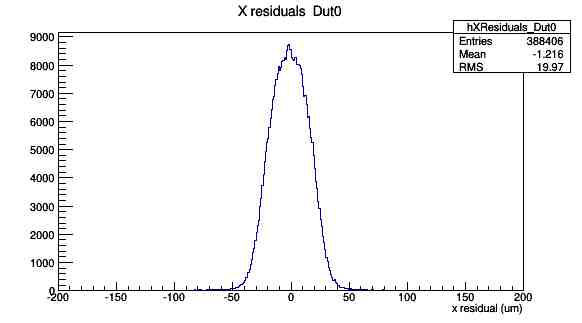
\includegraphics[width=0.6\textwidth]{ch8/ch8_img_X_res}
	\caption[X_residuals.] {X residuals.}
	\label{xres}
\end{figure}

\begin{figure}[!h]
	\centering
	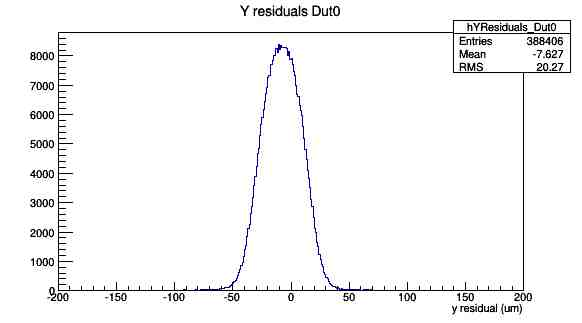
\includegraphics[width=0.6\textwidth]{ch8/ch8_img_Y_res}
	\caption[Y residuals.] {Y residuals.}
	\label{yres}
\end{figure}




%\section{Introduction}
%pixel from cms phase 0 2 by 4
%and strips from D0
%\section{The RD53 Chip}
%\section{Purpose of Test Beam}
%\section{Test Beam Set Up}
%\section{Results}
%\section{Conclusions and Future Work}